\documentclass[tikz,border=10pt]{standalone}
\begin{document}
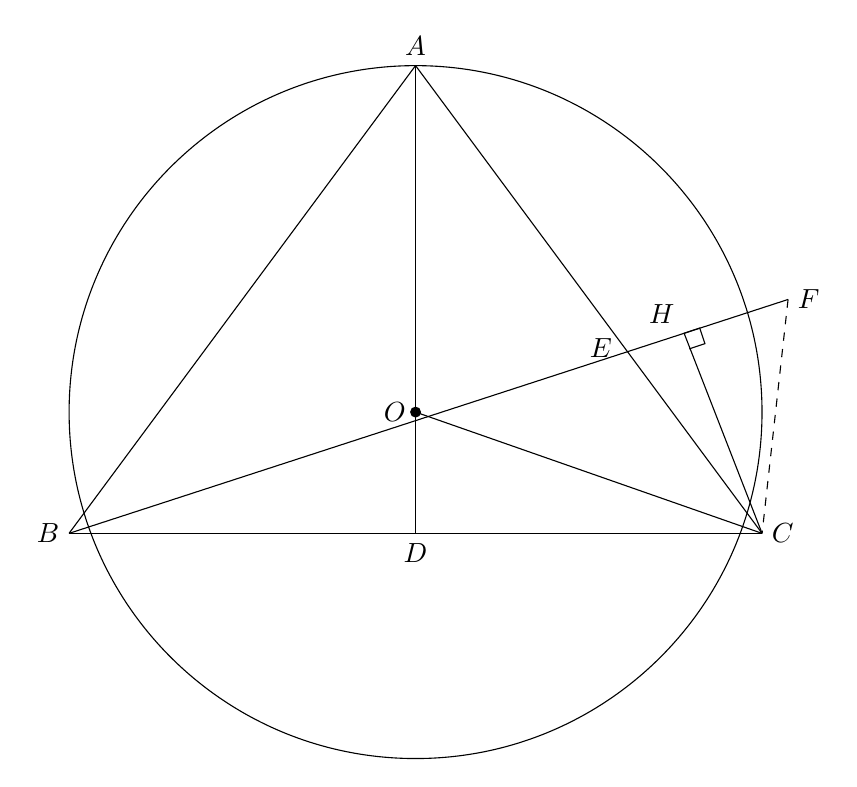
\begin{tikzpicture}[scale=1.1]

% Coordinates
\coordinate (O) at (0,0);
\coordinate (A) at (0,4);
\coordinate (B) at (-4,-1.4);
\coordinate (C) at (4,-1.4);
\coordinate (D) at (0,-1.4);
\coordinate (F) at (4.3,1.3);
\coordinate (E) at (1.9,0.52);
\coordinate (H) at (3.1,0.91);

% Circle through A, B, C
\draw (O) circle[radius=4];

% Main triangle and segments
\draw (A) -- (B);
\draw (A) -- (C);
\draw (B) -- (C);
\draw (A) -- (D);
\draw (B) -- (F);
\draw (O) -- (C);

% Interior/dashed segments on the right
\draw (H) -- (C);
\draw[dashed] (F) -- (C);

% Right-angle mark at H between HF and HC
\draw (H) -- ++(0.18,0.06) -- ++(0.06,-0.18) -- ++(-0.18,-0.06);

% Point markers
\fill (O) circle[radius=1.8pt];

% Labels
\node[above] at (A) {$A$};
\node[left] at (B) {$B$};
\node[right] at (C) {$C$};
\node[below] at (D) {$D$};
\node[above right] at (E) {$E$};
\node[right] at (F) {$F$};
\node[above left] at (H) {$H$};
\node[left] at (O) {$O$};

\end{tikzpicture}
\end{document}
